%\documentclass[mathserif]{beamer}
\documentclass[handout]{beamer}
%\usetheme{Goettingen}
\usetheme{Warsaw}
%\usetheme{Singapore}
%\usetheme{Frankfurt}
%\usetheme{Copenhagen}
%\usetheme{Szeged}
%\usetheme{Montpellier}
%\usetheme{CambridgeUS}
%\usecolortheme{}
%\setbeamercovered{transparent}
\usepackage[english, activeacute]{babel}
\usepackage[utf8]{inputenc}
\usepackage{amsmath, amssymb}
\usepackage{dsfont}
\usepackage{graphics}
\usepackage{cases}
\usepackage{graphicx}
\usepackage{pgf}
\usepackage{epsfig}
\usepackage{amssymb}
\usepackage{multirow}	
\usepackage{amstext}
\usepackage[ruled,vlined,lined]{algorithm2e}
\usepackage{amsmath}
\usepackage{epic}
\usepackage{epsfig}
\usepackage{fontenc}
\usepackage{framed,color}
\usepackage{palatino, url, multicol}
\usepackage{listings}
%\algsetup{indent=2em}
\newcommand{\factorial}{\ensuremath{\mbox{\sc Factorial}}}
\newcommand{\BIGOP}[1]{\mathop{\mathchoice%
{\raise-0.22em\hbox{\huge $#1$}}%
{\raise-0.05em\hbox{\L
\usepackage{fontenc}
\usepackage{framed,color}
\usepackage{palatino, url, multicol}
\usepackage{listings}
%\algsetup{indent=2em}
\newcommand{\factorial}{\ensuremath{\mbox{\sc Factorial}}}
\newcommand{\BIGOP}[1]{\mathop{\mathchoice%
{\raise-0.22em\hbox{\huge $#1$}}%
{\raise-0.05em\hbox{\Large $#1$}}{\hbox{\large $#1$}}{#1}}}
\newcommand{\bigtimes}{\BIGOP{\times}}
\vspace{-0.5cm}
\title{Introduction to Statistical Inference}
\vspace{-0.5cm}
\author[Felipe Bravo Márquez]{\footnotesize
%\author{\footnotesize  
 \textcolor[rgb]{0.00,0.00,1.00}{Felipe José Bravo Márquez}} 
\date{ \today }
arge $#1$}}{\hbox{\large $#1$}}{#1}}}
\newcommand{\bigtimes}{\BIGOP{\times}}
\vspace{-0.5cm}
\title{Introduction to Statistical Thinking}
\vspace{-0.5cm}
\author[Felipe Bravo Márquez]{\footnotesize
%\author{\footnotesize  
 \textcolor[rgb]{0.00,0.00,1.00}{Felipe José Bravo Márquez}} 
\date{ \today }


\begin{document}
\begin{frame}
\titlepage


\end{frame}


%%%%%%%%%%%%%%%%%%%%%%%%%%%


\begin{frame}{Introduction to Statistical Thinking}
\scriptsize{
\begin{itemize}
\item Statistical thinking is a systematic way of thinking about how we describe the \textbf{world} and use \textbf{data} make decisions and predictions.

\item Taking into account the inherent \textbf{uncertainty} that exists in the real world.  \cite{poldrack2019statistical}

 
 \item The foundations of statistical thinking come primarily from mathematics and statistics, but also from computer science, psychology, and other fields of study. \cite{poldrack2019statistical}
 
 \item \textbf{Statistics}, in particular, is the discipline that concerns the collection, organization, analysis, interpretation, and presentation of data \cite{wiki:Statistics}.
 
\end{itemize}

\begin{figure}[h!]
	\centering
	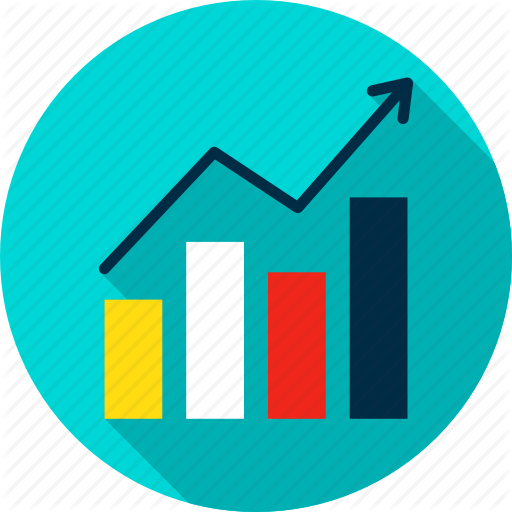
\includegraphics[scale=0.2]{pics/stats.png}
\end{figure}

} 
\end{frame}



\begin{frame}{Statistical Thinking and Intuition}

\scriptsize{
\begin{itemize}
\item Human \textbf{intuition} often tries to answer the same questions that we can answer using statistical thinking, but often gets the answer \textbf{wrong}. 
\item For example, in recent years most Americans have reported that they think that violent crime was worse compared to the previous year (Pew Research Center). 
\item However, a statistical analysis of the actual crime data shows that in fact violent crime has steadily decreased since the 1990’s. 
\item Intuition fails us because we rely upon \textbf{best guesses} (which psychologists refer to as heuristics) that can often get it wrong. \cite{poldrack2019statistical}


\end{itemize}

}
 
\end{frame}


\begin{frame}{What can statistics do for us?}
There are three major things that we can do with statistics:

\begin{itemize}
\item \textbf{Describe}: The world is complex and we often need to describe it in a simplified way that we can understand.
\item \textbf{Decide}: We often need to make decisions based on data, usually in the face of uncertainty.
\item \textbf{Predict}: We often wish to make predictions about new situations based on our knowledge of previous situations.



\end{itemize}


 
\end{frame}


\begin{frame}{Course Philosophy}

\scriptsize{
There two radical approaches to teach an introductory course on statistics.
\begin{block}{Mathematical Statistics}
 \begin{itemize}
\item This is usually taught in mathematics departments.
\item The focus is on the mathematical aspects of statistics (e.g., asymptotic properties).
\end{itemize}
\end{block}


\begin{block}{Applied Statistics}
 \begin{itemize}
\item This is usually taught in health and social science departments (e.g., psychology).
\item The focus in on the methods (e.g., t-test, ANOVA, linear regression) and how to apply them to the specific field.
\end{itemize}
\end{block}




}
 
\end{frame}

\begin{frame}{Course Philosophy}

\scriptsize{
 \begin{itemize}
\item In my personal opinion mathematical courses are in many cases hard to grasp for non-mathematical students and don't pay enough attention to the use of statistics in real world problems.
\item On the other hand, applied courses sometimes omit the fundamental assumptions on which the methods are based and end up being a kind of recipe book of methods for ad hoc problems. 

\item This course distinguishes itself from the two previous paradigms by focusing on the understanding of the basic ideas of statistical thinking.

\item We will reflect on the assumptions on which the different models are based, and we will be aware that no method or tool fits perfectly to every problem.

\end{itemize}



}
 
\end{frame}


\begin{frame}{Example of flowchart (recipe book) taken from \cite{mcelreath2020statistical}} 


\begin{figure}[h!]
	\centering
	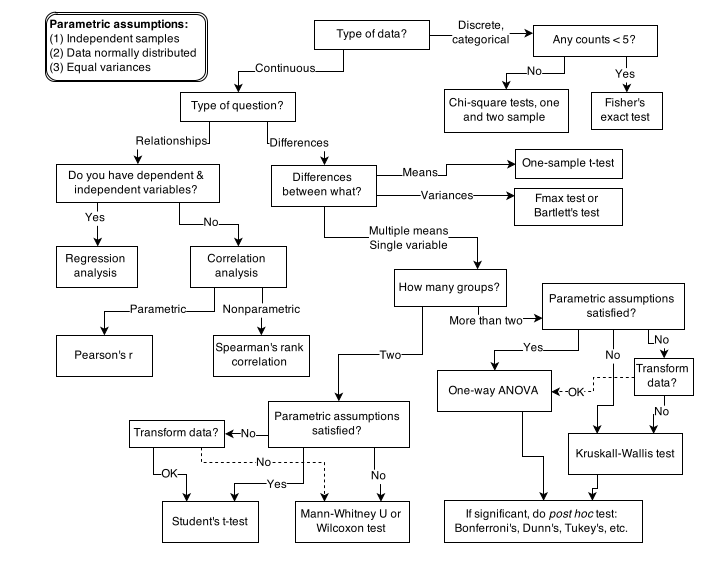
\includegraphics[scale=0.38]{pics/flowchart.png}
\end{figure}


 
\end{frame}

\begin{frame}{Roadmap}

\scriptsize{
The main topics that will be covered in this course are:
\begin{itemize}
\item Statistical Programing in R
\item Descriptive Statistics
\item Probability
\item Frequentist Inference
\item Bayesian Inferece
\end{itemize}

}
 
\end{frame}


%%%%%%%%%%%%%%%%%%%%%%%%%%%
\begin{frame}[allowframebreaks]\scriptsize
\frametitle{References}
\bibliography{bio}
\bibliographystyle{apalike}
%\bibliographystyle{flexbib}
\end{frame}  









%%%%%%%%%%%%%%%%%%%%%%%%%%%

\end{document}
